\documentclass[]{article}
\usepackage{lmodern}
\usepackage{amssymb,amsmath}
\usepackage{ifxetex,ifluatex}
\usepackage{fixltx2e} % provides \textsubscript
\ifnum 0\ifxetex 1\fi\ifluatex 1\fi=0 % if pdftex
  \usepackage[T1]{fontenc}
  \usepackage[utf8]{inputenc}
\else % if luatex or xelatex
  \ifxetex
    \usepackage{mathspec}
  \else
    \usepackage{fontspec}
  \fi
  \defaultfontfeatures{Ligatures=TeX,Scale=MatchLowercase}
\fi
% use upquote if available, for straight quotes in verbatim environments
\IfFileExists{upquote.sty}{\usepackage{upquote}}{}
% use microtype if available
\IfFileExists{microtype.sty}{%
\usepackage{microtype}
\UseMicrotypeSet[protrusion]{basicmath} % disable protrusion for tt fonts
}{}
\usepackage[margin=1in]{geometry}
\usepackage{hyperref}
\hypersetup{unicode=true,
            pdfborder={0 0 0},
            breaklinks=true}
\urlstyle{same}  % don't use monospace font for urls
\usepackage{color}
\usepackage{fancyvrb}
\newcommand{\VerbBar}{|}
\newcommand{\VERB}{\Verb[commandchars=\\\{\}]}
\DefineVerbatimEnvironment{Highlighting}{Verbatim}{commandchars=\\\{\}}
% Add ',fontsize=\small' for more characters per line
\usepackage{framed}
\definecolor{shadecolor}{RGB}{248,248,248}
\newenvironment{Shaded}{\begin{snugshade}}{\end{snugshade}}
\newcommand{\KeywordTok}[1]{\textcolor[rgb]{0.13,0.29,0.53}{\textbf{#1}}}
\newcommand{\DataTypeTok}[1]{\textcolor[rgb]{0.13,0.29,0.53}{#1}}
\newcommand{\DecValTok}[1]{\textcolor[rgb]{0.00,0.00,0.81}{#1}}
\newcommand{\BaseNTok}[1]{\textcolor[rgb]{0.00,0.00,0.81}{#1}}
\newcommand{\FloatTok}[1]{\textcolor[rgb]{0.00,0.00,0.81}{#1}}
\newcommand{\ConstantTok}[1]{\textcolor[rgb]{0.00,0.00,0.00}{#1}}
\newcommand{\CharTok}[1]{\textcolor[rgb]{0.31,0.60,0.02}{#1}}
\newcommand{\SpecialCharTok}[1]{\textcolor[rgb]{0.00,0.00,0.00}{#1}}
\newcommand{\StringTok}[1]{\textcolor[rgb]{0.31,0.60,0.02}{#1}}
\newcommand{\VerbatimStringTok}[1]{\textcolor[rgb]{0.31,0.60,0.02}{#1}}
\newcommand{\SpecialStringTok}[1]{\textcolor[rgb]{0.31,0.60,0.02}{#1}}
\newcommand{\ImportTok}[1]{#1}
\newcommand{\CommentTok}[1]{\textcolor[rgb]{0.56,0.35,0.01}{\textit{#1}}}
\newcommand{\DocumentationTok}[1]{\textcolor[rgb]{0.56,0.35,0.01}{\textbf{\textit{#1}}}}
\newcommand{\AnnotationTok}[1]{\textcolor[rgb]{0.56,0.35,0.01}{\textbf{\textit{#1}}}}
\newcommand{\CommentVarTok}[1]{\textcolor[rgb]{0.56,0.35,0.01}{\textbf{\textit{#1}}}}
\newcommand{\OtherTok}[1]{\textcolor[rgb]{0.56,0.35,0.01}{#1}}
\newcommand{\FunctionTok}[1]{\textcolor[rgb]{0.00,0.00,0.00}{#1}}
\newcommand{\VariableTok}[1]{\textcolor[rgb]{0.00,0.00,0.00}{#1}}
\newcommand{\ControlFlowTok}[1]{\textcolor[rgb]{0.13,0.29,0.53}{\textbf{#1}}}
\newcommand{\OperatorTok}[1]{\textcolor[rgb]{0.81,0.36,0.00}{\textbf{#1}}}
\newcommand{\BuiltInTok}[1]{#1}
\newcommand{\ExtensionTok}[1]{#1}
\newcommand{\PreprocessorTok}[1]{\textcolor[rgb]{0.56,0.35,0.01}{\textit{#1}}}
\newcommand{\AttributeTok}[1]{\textcolor[rgb]{0.77,0.63,0.00}{#1}}
\newcommand{\RegionMarkerTok}[1]{#1}
\newcommand{\InformationTok}[1]{\textcolor[rgb]{0.56,0.35,0.01}{\textbf{\textit{#1}}}}
\newcommand{\WarningTok}[1]{\textcolor[rgb]{0.56,0.35,0.01}{\textbf{\textit{#1}}}}
\newcommand{\AlertTok}[1]{\textcolor[rgb]{0.94,0.16,0.16}{#1}}
\newcommand{\ErrorTok}[1]{\textcolor[rgb]{0.64,0.00,0.00}{\textbf{#1}}}
\newcommand{\NormalTok}[1]{#1}
\usepackage{longtable,booktabs}
\usepackage{graphicx,grffile}
\makeatletter
\def\maxwidth{\ifdim\Gin@nat@width>\linewidth\linewidth\else\Gin@nat@width\fi}
\def\maxheight{\ifdim\Gin@nat@height>\textheight\textheight\else\Gin@nat@height\fi}
\makeatother
% Scale images if necessary, so that they will not overflow the page
% margins by default, and it is still possible to overwrite the defaults
% using explicit options in \includegraphics[width, height, ...]{}
\setkeys{Gin}{width=\maxwidth,height=\maxheight,keepaspectratio}
\IfFileExists{parskip.sty}{%
\usepackage{parskip}
}{% else
\setlength{\parindent}{0pt}
\setlength{\parskip}{6pt plus 2pt minus 1pt}
}
\setlength{\emergencystretch}{3em}  % prevent overfull lines
\providecommand{\tightlist}{%
  \setlength{\itemsep}{0pt}\setlength{\parskip}{0pt}}
\setcounter{secnumdepth}{0}
% Redefines (sub)paragraphs to behave more like sections
\ifx\paragraph\undefined\else
\let\oldparagraph\paragraph
\renewcommand{\paragraph}[1]{\oldparagraph{#1}\mbox{}}
\fi
\ifx\subparagraph\undefined\else
\let\oldsubparagraph\subparagraph
\renewcommand{\subparagraph}[1]{\oldsubparagraph{#1}\mbox{}}
\fi

%%% Use protect on footnotes to avoid problems with footnotes in titles
\let\rmarkdownfootnote\footnote%
\def\footnote{\protect\rmarkdownfootnote}

%%% Change title format to be more compact
\usepackage{titling}

% Create subtitle command for use in maketitle
\providecommand{\subtitle}[1]{
  \posttitle{
    \begin{center}\large#1\end{center}
    }
}

\setlength{\droptitle}{-2em}

  \title{}
    \pretitle{\vspace{\droptitle}}
  \posttitle{}
    \author{}
    \preauthor{}\postauthor{}
    \date{}
    \predate{}\postdate{}
  

\begin{document}

\begin{longtable}[]{@{}l@{}}
\toprule
tle: ``Duomenų analizės įvadas''\tabularnewline
btitle: `3.1.. dalis - R programavimas'\tabularnewline
thor: ``Justas Mundeikis''\tabularnewline
stitute: ``VU EVAF''\tabularnewline
te: ``2019-05-08''\tabularnewline
tput:\tabularnewline
eamer\_presentation:\tabularnewline
includes:\tabularnewline
in\_header: header.txt\tabularnewline
itor\_options:\tabularnewline
chunk\_output\_type: console\tabularnewline
\bottomrule
\end{longtable}

\subsection{Turinys}\label{turinys}

\tableofcontents

\section{Natūralūs vs apdoroti
duomenys}\label{naturalus-vs-apdoroti-duomenys}

\subsection{Intro}\label{intro}

Natūralūs duomenys (raw data) -\textgreater{} aprodojimo skriptas
-\textgreater{} tvarkingi duomenys -\textgreater{} duomenų analizė
-\textgreater{} komunikacija

\subsection{Natūralūs vs apdoroti
duomenys}\label{naturalus-vs-apdoroti-duomenys-1}

Natūralūs duomenys:

\begin{itemize}
\tightlist
\item
  Paimti iš duomenų šaltinio
\item
  Ne retai sunkiai pritaikomi analizei
\item
  Duomenų analizė ne retai apima ir duomenų apdorojimą
\item
  Natūralius duomenis gali reikėti apdoroti vieną ar kelis kartus
  \href{https://en.wikipedia.org/wiki/Raw_data}{wiki:Raw\_data}
\end{itemize}

Apdoroti duomenys:

\begin{itemize}
\tightlist
\item
  Duomenys paruošti analizei
\item
  Apdorojimas gali apimti duomenų apjungimą, dalinimą, transformavimą
  etc.
\item
  Priklausomai nuo aplinkybių, gali egzistuoti duomenų aprodojimo
  standartai
\item
  Visi duomenų apdorojimo žingsniai turi būti dokumentuoti
\end{itemize}

\subsection{Raw to tidy}\label{raw-to-tidy}

\begin{enumerate}
\def\labelenumi{\arabic{enumi}.}
\tightlist
\item
  Natūralūs duomenys (raw data set)
\item
  Tvarkingi duomenys (tidy data set)
\item
  \emph{Code book} (meta doumenys) tvarkingiems duomenims
\item
  R Skriptas (1.-\textgreater{} 2.)
\end{enumerate}

\subsection{Tvarkingi duomenys}\label{tvarkingi-duomenys}

\begin{enumerate}
\def\labelenumi{\arabic{enumi}.}
\tightlist
\item
  Vienas kintamasis - 1 stuleplis
\item
  Viena observacija - 1 eilutė
\item
  Vienam kintamajam - 1 lentelė
\item
  Daug lentelių gali būti sujungtos per vieną stulpelį
\item
  Pirma eilutė - žmonėms suprantami kintamųjų pavadinimai (Pajamos vs
  Pj)
\item
  Viena lentelė - vienas failas
\end{enumerate}

\subsection{Code book}\label{code-book}

\begin{enumerate}
\def\labelenumi{\arabic{enumi}.}
\tightlist
\item
  Informacija apie kintamuosus, jų matavimo vienetus (gali nebūti
  apdorotuose duomenyse)
\item
  Informacija, kaip surinkti duomenys (apklausos metodai\ldots{})
\item
  Informacija, kaip apdoroti duomenys
\item
  Pageidautina .txt failas su markdown sintakse
\end{enumerate}

\subsection{Duomenų apdorojimo
skriptas}\label{duomenu-apdorojimo-skriptas}

\begin{itemize}
\tightlist
\item
  Duomenų apdrorojimo skriptas R, Python, Stata, SPSS
\item
  Turi priimti natūralius duomenis
\item
  Grąžinti tvarkingus duomenis
\item
  Skripte neturėtų būti jokių nuo vartotojo priklausomų parametrų /
  nustatymų
\item
  Jeigu skripte neįmanoma automatiškai atlikti visų veiksmų, būtina
  detaliai aprašyti (codebook + skripte komentavimo funckija)
\end{itemize}

\subsection{Kas būna kai\ldots{}}\label{kas-buna-kai}

Does high public debt consistently stifle economic growth? A critique of
Reinhart and Rogoff

We replicate Reinhart and Rogoff (2010A and 2010B) and find that
selective exclusion of available data, coding errors and inappropriate
weighting of summary statistics lead to serious miscalculations that
inaccurately represent the relationship between public debt and GDP
growth among 20 advanced economies. Over 1946--2009, countries with
public debt/GDP ratios above 90\% averaged 2.2\% real annual GDP growth,
not −0.1\% as published\ldots{}

\href{https://umassmed.edu/globalassets/quantitative-health-sciences/files/camb.-j.-econ.-2013-herndon-cje-bet075.pdf}{Does
high public debt consistently stifle economic growth? A critique of
Reinhart and Rogoff}

\subsection{Darbinė direktorija}\label{darbine-direktorija}

\begin{itemize}
\tightlist
\item
  \texttt{getwd()} ir \texttt{setwd()}
\item
  relatyvus adresas \texttt{setwd("./data")}, \texttt{setwd("../data")}
\item
  absoliutus adresas
  \texttt{setwd(c:/users/studentas/desktop/test/data)}
\item
  nenaudokite absoliučių adresų
\item
  INSTR: pakeisti darbinę direkrotiją į ``Desktop''
\end{itemize}

\subsection{Darbinė direktorija}\label{darbine-direktorija-1}

\begin{itemize}
\tightlist
\item
  \texttt{file.exists("file\_name")} testuoja ar egzistuoja failas arba
  direktorija
\item
  \texttt{dir.create("folder\_name")} sukuria direktoriją
\item
  jeigu skriptas importuoja duomenis, o duomenys turi būti patalpinti
  atksiroje direktorijoje:
\end{itemize}

\begin{Shaded}
\begin{Highlighting}[]
\ControlFlowTok{if}\NormalTok{(}\OperatorTok{!}\KeywordTok{file.exists}\NormalTok{(}\StringTok{"data"}\NormalTok{))\{}
        \KeywordTok{dir.create}\NormalTok{(}\StringTok{"data"}\NormalTok{)}
\NormalTok{\}}
\end{Highlighting}
\end{Shaded}

\subsection{\texorpdfstring{\texttt{paste()}}{paste()}}\label{paste}

\begin{itemize}
\tightlist
\item
  \texttt{paste()} funkcija sujungia stringus / vectorius į vieną
  \emph{character} string
\end{itemize}

\begin{Shaded}
\begin{Highlighting}[]
\NormalTok{times <-}\StringTok{"Times"}\NormalTok{; x <-}\StringTok{ }\DecValTok{3}
\KeywordTok{paste}\NormalTok{(}\StringTok{"Hello"}\NormalTok{, }\StringTok{"World"}\NormalTok{, x, times, }\DataTypeTok{sep=}\StringTok{" "}\NormalTok{)}
\NormalTok{## [1] "Hello World 3 Times"}
\KeywordTok{paste}\NormalTok{(}\StringTok{"Hello"}\NormalTok{, }\StringTok{"World"}\NormalTok{, x, times , }\DataTypeTok{sep =} \StringTok{"_"}\NormalTok{)}
\NormalTok{## [1] "Hello_World_3_Times"}
\NormalTok{a <-}\StringTok{ }\KeywordTok{c}\NormalTok{(}\DecValTok{1}\NormalTok{,}\DecValTok{2}\NormalTok{,}\DecValTok{3}\NormalTok{,}\DecValTok{4}\NormalTok{); b <-}\StringTok{ }\KeywordTok{c}\NormalTok{(}\StringTok{"a"}\NormalTok{, }\StringTok{"b"}\NormalTok{, }\StringTok{"c"}\NormalTok{)}
\KeywordTok{paste}\NormalTok{(a,b, }\DataTypeTok{sep=}\StringTok{"&"}\NormalTok{, }\DataTypeTok{collapse=}\StringTok{"%"}\NormalTok{)}
\NormalTok{## [1] "1&a%2&b%3&c%4&a"}
\end{Highlighting}
\end{Shaded}

\section{Duomenys iš interneto}\label{duomenys-is-interneto}

\subsection{Duomenys iš interneto}\label{duomenys-is-interneto-1}

\begin{itemize}
\tightlist
\item
  \texttt{download.file(url,\ destfile,\ method,\ quiet\ =\ FALSE,\ mode\ =\ "w",\ cacheOK\ =\ TRUE,\ extra\ =\ getOption("download.file.extra"))}
\item
  tinka duomenų failų parsiuntimui (.txt, .csv, etc)
\item
  Keliaujam į \url{http://atvira.sodra.lt/lt-eur/} - Apdraustieji -
  Vidutinių apdraustųjų pajamų analizė - CSV
\item
  Nusikopijuojam url 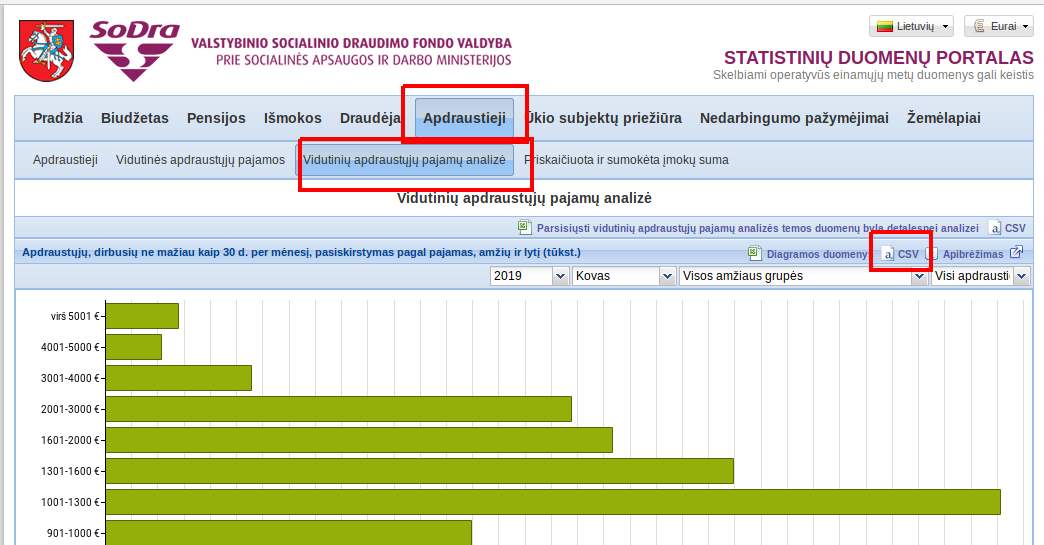
\includegraphics{./figures/sodra_1.png}
\end{itemize}

\subsection{Duomenys iš interneto}\label{duomenys-is-interneto-2}

\begin{Shaded}
\begin{Highlighting}[]
\NormalTok{URL <-}\StringTok{ "http://atvira.sodra.lt/csv/lt-eur/apdraustieji_3_1.csv"}
\KeywordTok{Sys.time}\NormalTok{()}
\NormalTok{DownloadDate <-}\StringTok{ }\KeywordTok{format}\NormalTok{(}\KeywordTok{Sys.time}\NormalTok{(), }\DataTypeTok{format=}\StringTok{"%Y_%m_%d"}\NormalTok{)}
\NormalTok{filename <-}\StringTok{ }\KeywordTok{paste}\NormalTok{(}\StringTok{"./data/apdraustieji_3_1_"}\NormalTok{,}
\NormalTok{                         DownloadDate,}
                         \StringTok{".csv"}\NormalTok{, }
                         \DataTypeTok{sep =} \StringTok{""}\NormalTok{)}
\NormalTok{filename}
\CommentTok{# pastaba: method="curl" arba "wininet" kartais veikia geriau, svarbu išsibandyti}
\KeywordTok{download.file}\NormalTok{(}
        \DataTypeTok{url =}\NormalTok{ URL, }
        \DataTypeTok{destfile =}\NormalTok{ filename, }
        \DataTypeTok{method =} \StringTok{"auto"}\NormalTok{)}
\end{Highlighting}
\end{Shaded}

\subsection{Duomenys iš interneto}\label{duomenys-is-interneto-3}

\begin{itemize}
\tightlist
\item
  Dabar visą zip failą ``apdraustuju\_pajamu\_analize.zip''
\end{itemize}

\begin{Shaded}
\begin{Highlighting}[]
\NormalTok{URL <-}\StringTok{ "http://atvira.sodra.lt/downloads/lt-eur/apdraustuju_pajamu_analize.zip"}
\NormalTok{DownloadDate <-}\StringTok{ }\KeywordTok{format}\NormalTok{(}\KeywordTok{Sys.time}\NormalTok{(), }\DataTypeTok{format=}\StringTok{"%Y_%m_%d"}\NormalTok{)}
\NormalTok{filename <-}\StringTok{ }\KeywordTok{paste}\NormalTok{(}\StringTok{"./data/apdraustuju_pajamu_analize_"}\NormalTok{,}
\NormalTok{                         DownloadDate,}
                         \StringTok{".zip"}\NormalTok{, }
                         \DataTypeTok{sep =} \StringTok{""}\NormalTok{)}
\NormalTok{filename}
\KeywordTok{download.file}\NormalTok{(}
        \DataTypeTok{url =}\NormalTok{ URL, }
        \DataTypeTok{destfile =}\NormalTok{ filename,}
        \DataTypeTok{method =} \StringTok{"auto"}\NormalTok{)}

\CommentTok{# jeigu daugiau nei vienas failas, nurodyti tikslų failo pavadinimą}
\KeywordTok{unzip}\NormalTok{(filename,}
      \DataTypeTok{exdir=}\StringTok{"data"}\NormalTok{,}
      \DataTypeTok{files =} \StringTok{"apdraustuju_pajamu_analize.csv"}\NormalTok{)}
\end{Highlighting}
\end{Shaded}

\subsection{Duomenys iš interneto}\label{duomenys-is-interneto-4}

\begin{itemize}
\tightlist
\item
  sukuriamas \texttt{temp()} failas
\item
  į jį nudownloadinamas failas
\item
  iš temp failo išsiekstrahuojame reikiamą turinį
\item
  kai nebereikia \texttt{unlink(...)} panaikina \texttt{temp()} failą
\end{itemize}

\begin{Shaded}
\begin{Highlighting}[]
\NormalTok{URL <-}\StringTok{ "http://atvira.sodra.lt/downloads/lt-eur/apdraustuju_pajamu_analize.zip"}
\NormalTok{temp <-}\StringTok{ }\KeywordTok{tempfile}\NormalTok{()}
\KeywordTok{download.file}\NormalTok{(}\DataTypeTok{url =}\NormalTok{ URL, temp, }\DataTypeTok{method =} \StringTok{"auto"}\NormalTok{)}
\NormalTok{GYV_PAJ <-}\StringTok{ }\KeywordTok{read.csv}\NormalTok{(}\KeywordTok{unzip}\NormalTok{(temp,}\StringTok{"apdraustuju_pajamu_analize.csv"}\NormalTok{),}
                 \DataTypeTok{header=}\OtherTok{TRUE}\NormalTok{,}
                 \DataTypeTok{sep=}\StringTok{";"}\NormalTok{,}
                 \DataTypeTok{stringsAsFactors =} \OtherTok{FALSE}\NormalTok{) }
\KeywordTok{unlink}\NormalTok{(temp)}
\end{Highlighting}
\end{Shaded}

\subsection{Duomenys iš interneto}\label{duomenys-is-interneto-5}

\begin{Shaded}
\begin{Highlighting}[]
\KeywordTok{median}\NormalTok{(GYV_PAJ}\OperatorTok{$}\NormalTok{Mėnesio.pajamos)}
\KeywordTok{list}\NormalTok{(}\DataTypeTok{lower_bound =} \FloatTok{0.5}\OperatorTok{*}\KeywordTok{median}\NormalTok{(GYV_PAJ}\OperatorTok{$}\NormalTok{Mėnesio.pajamos),}
\DataTypeTok{median=} \KeywordTok{median}\NormalTok{(GYV_PAJ}\OperatorTok{$}\NormalTok{Mėnesio.pajamos),}
\DataTypeTok{upper_bound =} \DecValTok{2}\OperatorTok{*}\KeywordTok{median}\NormalTok{(GYV_PAJ}\OperatorTok{$}\NormalTok{Mėnesio.pajamos))}

\NormalTok{maximum <-}\StringTok{ }\DecValTok{4000}
\KeywordTok{hist}\NormalTok{(GYV_PAJ}\OperatorTok{$}\NormalTok{Mėnesio.pajamos[GYV_PAJ}\OperatorTok{$}\NormalTok{Mėnesio.pajamos}\OperatorTok{<=}\NormalTok{maximum],}
     \DataTypeTok{main=}\StringTok{"Histogram of declared labor income"}\NormalTok{,}
     \DataTypeTok{xlab=}\StringTok{"Income grouped by 100"}\NormalTok{,}
     \DataTypeTok{breaks=}\KeywordTok{seq}\NormalTok{(}\DecValTok{0}\NormalTok{,maximum,}\DecValTok{100}\NormalTok{),}
     \DataTypeTok{xaxt=}\StringTok{"n"}\NormalTok{)}
\KeywordTok{axis}\NormalTok{(}\DataTypeTok{side=}\DecValTok{1}\NormalTok{, }\DataTypeTok{at=}\KeywordTok{seq}\NormalTok{(}\DecValTok{0}\NormalTok{,maximum, }\DecValTok{100}\NormalTok{), }\DataTypeTok{labels=}\KeywordTok{seq}\NormalTok{(}\DecValTok{0}\NormalTok{,maximum,}\DecValTok{100}\NormalTok{))}
\end{Highlighting}
\end{Shaded}

\subsection{Duomenys iš interneto}\label{duomenys-is-interneto-6}

\begin{itemize}
\tightlist
\item
  100\% tikrumo, koks failo \texttt{encoding} neduos niekas
\item
  Geras būdas, pabandyti atsidaryti su LibreOffice Calc, Sublime
\item
  Mažiau tiksli alternatyva \texttt{guess\_encoding} iš paketo
  \texttt{readr}
\item
  google
\end{itemize}

\begin{Shaded}
\begin{Highlighting}[]
\CommentTok{#install.packages("readr")}
\KeywordTok{library}\NormalTok{(readr)}
\KeywordTok{guess_encoding}\NormalTok{(}\StringTok{"./data/apdraustuju_pajamu_analize.csv"}\NormalTok{, }\DataTypeTok{n_max =} \DecValTok{1000}\NormalTok{)}
\NormalTok{## # A tibble: 3 x 2}
\NormalTok{##   encoding   confidence}
\NormalTok{##   <chr>           <dbl>}
\NormalTok{## 1 ISO-8859-1       0.63}
\NormalTok{## 2 ISO-8859-2       0.41}
\NormalTok{## 3 ISO-8859-9       0.22}
\end{Highlighting}
\end{Shaded}

\subsection{Duomenu nuskaitymas}\label{duomenu-nuskaitymas}

\begin{itemize}
\tightlist
\item
  \texttt{read.table}
\item
  \texttt{read.csv} , \texttt{read.csv2}, etc
\item
  \texttt{readr} importavimo tool'sas (generuoja R kodą)
\end{itemize}

\begin{Shaded}
\begin{Highlighting}[]
\NormalTok{df <-}\StringTok{ }\KeywordTok{read.table}\NormalTok{(}\StringTok{"./data/apdraustuju_pajamu_analize.csv"}\NormalTok{,}
                 \DataTypeTok{header=}\OtherTok{TRUE}\NormalTok{,}
                 \DataTypeTok{sep=}\StringTok{";"}\NormalTok{,}
                 \DataTypeTok{fileEncoding =} \StringTok{"ISO-8859-13"}\NormalTok{,}
                 \DataTypeTok{stringsAsFactors =} \OtherTok{FALSE}\NormalTok{) }
\end{Highlighting}
\end{Shaded}

\subsection{Galvos skausmas Excel
formatai}\label{galvos-skausmas-excel-formatai}

\begin{itemize}
\tightlist
\item
  iš Sodros
\item
  parsisiunčiam \texttt{.xlsx} failą
\end{itemize}

\begin{Shaded}
\begin{Highlighting}[]
\NormalTok{URL <-}\StringTok{ }
\StringTok{"http://atvira.sodra.lt/downloads/lt-eur/apdraustuju_pajamu_analize.xlsx"}
\NormalTok{DownloadDate <-}\StringTok{ }\KeywordTok{format}\NormalTok{(}\KeywordTok{Sys.time}\NormalTok{(), }\DataTypeTok{format=}\StringTok{"%Y_%m_%d"}\NormalTok{)}
\KeywordTok{download.file}\NormalTok{(}\DataTypeTok{url =}\NormalTok{ URL, }
              \DataTypeTok{destfile =} \KeywordTok{paste}\NormalTok{(}\StringTok{"./data/apdraustuju_pajamu_analize_"}\NormalTok{,}
\NormalTok{                               DownloadDate,}
                               \StringTok{".xlsx"}\NormalTok{, }
                               \DataTypeTok{sep =} \StringTok{""}\NormalTok{), }
              \DataTypeTok{method =} \StringTok{"auto"}\NormalTok{)}
\end{Highlighting}
\end{Shaded}

\subsection{Galvos skausmas Excel
formatai}\label{galvos-skausmas-excel-formatai-1}

\begin{itemize}
\tightlist
\item
  \texttt{readxl} paketas
\item
  \texttt{xlsx} paketas
\item
  alternatyva atsidaryti su Excel, išsaugoti kaip \texttt{.csv},
  importuoti kaip \texttt{.csv}
\end{itemize}

\begin{Shaded}
\begin{Highlighting}[]
\CommentTok{#install.packages("readxl")}
\KeywordTok{library}\NormalTok{(readxl)}
\CommentTok{# su Excel pasitikriname, kurį sheet importuosime}
\NormalTok{df2 <-}\StringTok{ }\KeywordTok{read_excel}\NormalTok{(}\StringTok{".data/apdraustuju_pajamu_analize_2019_05_08.xlsx"}\NormalTok{, }
                  \DataTypeTok{sheet =} \StringTok{"Duomenys"}\NormalTok{)}
\KeywordTok{str}\NormalTok{(df2)}
\end{Highlighting}
\end{Shaded}

\subsection{Galvos skausmas Excel
formatai}\label{galvos-skausmas-excel-formatai-2}

\begin{itemize}
\tightlist
\item
  \texttt{write\_excel\_csv()} su \texttt{readr} paketu
\item
  \texttt{write.xlsx} su \texttt{openxlsx} paketu
\item
  SVARBU! Excel neatidaro daugiau nei
\item
  1 048 57 eilučių ir 16 384 stulpelių
\end{itemize}

\begin{Shaded}
\begin{Highlighting}[]
\KeywordTok{install.packages}\NormalTok{(}\StringTok{"openxlsx"}\NormalTok{)}
\KeywordTok{library}\NormalTok{(openxlsx)}
\NormalTok{l<-}\KeywordTok{list}\NormalTok{(}\DataTypeTok{iris=}\NormalTok{iris, }\DataTypeTok{mtcars=}\NormalTok{mtcars, }\DataTypeTok{quakes=}\NormalTok{quakes)}
\KeywordTok{write.xlsx}\NormalTok{(l, }\DataTypeTok{file =} \StringTok{"./data/datasets.xlsx"}\NormalTok{)}
\end{Highlighting}
\end{Shaded}

\subsection{LSD}\label{lsd}

\begin{itemize}
\tightlist
\item
  LSD sukelia daug galvos skausmų, tačiau LSD turi API
\item
  \href{https://osp.stat.gov.lt/rdb-rest}{``RESTful žiniatinklio
  paslaugos''} *\texttt{rsdmx} paketas sutvarko LSD failus
\end{itemize}

\begin{Shaded}
\begin{Highlighting}[]
\CommentTok{#install.packages("rsdmx")}
\KeywordTok{library}\NormalTok{(rsdmx)}
\end{Highlighting}
\end{Shaded}

\subsection{LSD}\label{lsd-1}

Pavyzdžiai: * kai norima gauti duomenų rinkinių sąrašą *
\url{https://osp-rs.stat.gov.lt/rest_xml/dataflow/} * kai norima gauti
konkretaus duomenų rinkinio apibrėžimą *
\url{https://osp-rs.stat.gov.lt/rest_xml/dataflow/LSD/S3R629_M3010217} *
kai norima gauti duomenų struktūros apibrėžimą *
\url{https://osp-rs.stat.gov.lt/rest_xml/datastructure/lsd/M3010217/}

\begin{Shaded}
\begin{Highlighting}[]
\CommentTok{#metadata}
\NormalTok{url_meta <-}\StringTok{ "https://osp-rs.stat.gov.lt/rest_xml/dataflow/"}

\NormalTok{meta <-}\StringTok{ }\KeywordTok{readSDMX}\NormalTok{(url_meta)}
\NormalTok{meta <-}\StringTok{ }\KeywordTok{as.data.frame}\NormalTok{(meta)}

\KeywordTok{write.csv}\NormalTok{(meta, }\StringTok{"./data/meta.csv"}\NormalTok{)}
\KeywordTok{write.xlsx}\NormalTok{(meta, }\DataTypeTok{file =} \StringTok{"./data/meta.xlsx"}\NormalTok{)}
\end{Highlighting}
\end{Shaded}

\subsection{LSD}\label{lsd-2}

\begin{itemize}
\tightlist
\item
  išsirinkus kokio kintamojo reikia
\end{itemize}

\begin{Shaded}
\begin{Highlighting}[]
\CommentTok{# S3R838 - Deaths by cause of death}
\CommentTok{# Age (5 year groups) | Causes of death (27) | Sex (2000 - 2016)}
\NormalTok{S3R838_M3010608<-}\StringTok{ }\KeywordTok{readSDMX}\NormalTok{(}\DataTypeTok{providerId =} \StringTok{"LSD"}\NormalTok{, }
                           \DataTypeTok{resource =} \StringTok{"data"}\NormalTok{, }
                           \DataTypeTok{flowRef =} \StringTok{"S3R838_M3010608"}\NormalTok{, }
                           \DataTypeTok{dsd =} \OtherTok{TRUE}\NormalTok{)}
\NormalTok{## -> Fetching 'https://osp-rs.stat.gov.lt/rest_xml/data/S3R838_M3010608/all/'}
\NormalTok{## -> DSD ref identified in dataset = 'M3010608'}
\NormalTok{## -> Attempt to fetch & bind DSD to dataset}
\NormalTok{## -> Fetching 'https://osp-rs.stat.gov.lt/rest_xml/datastructure/all/M3010608/latest/?references=children'}
\NormalTok{## -> DSD fetched and associated to dataset!}
\NormalTok{S3R838_M3010608 <-}\StringTok{ }\KeywordTok{as.data.frame}\NormalTok{(S3R838_M3010608 , }
                                 \DataTypeTok{labels =} \OtherTok{TRUE}\NormalTok{)}
\end{Highlighting}
\end{Shaded}

\subsection{RSDMX}\label{rsdmx}

\begin{itemize}
\tightlist
\item
  padeda imporuoti ir duomenis iš OECD, Eurostat ir kitų šaltinių,
  kuriuose duomenys pateikiami XML formatu
\item
  žr. \url{https://github.com/opensdmx/rsdmx}
\end{itemize}

\subsection{Eurostat}\label{eurostat}

\begin{itemize}
\tightlist
\item
  \texttt{eurostat} paketas
\item
  google ``eurostat cheatsheet''
\item
  einam į Eurostat database išsirinkt duomenų\ldots{}
\end{itemize}

\begin{Shaded}
\begin{Highlighting}[]
\CommentTok{#install.packages("eurostat")}
\KeywordTok{library}\NormalTok{(eurostat)}
\NormalTok{nama_10_gdp <-}\StringTok{ }\KeywordTok{get_eurostat}\NormalTok{(}\StringTok{"nama_10_gdp"}\NormalTok{, }\DataTypeTok{stringsAsFactors =} \OtherTok{FALSE}\NormalTok{)}
\end{Highlighting}
\end{Shaded}

\section{Duomenų inspektavimas}\label{duomenu-inspektavimas}

\subsection{Inspection}\label{inspection}

\begin{Shaded}
\begin{Highlighting}[]
\KeywordTok{head}\NormalTok{(df,}\DecValTok{2}\NormalTok{)}
\NormalTok{##   Metai Menuo Amžius   Lytis Menesio.pajamos}
\NormalTok{## 1  2019     3     39 Moteris         4124.80}
\NormalTok{## 2  2019     3     55 Moteris          861.56}
\KeywordTok{tail}\NormalTok{(df,}\DecValTok{2}\NormalTok{)}
\NormalTok{##         Metai Menuo Amžius   Lytis Menesio.pajamos}
\NormalTok{## 1108113  2019     3     36   Vyras         1528.95}
\NormalTok{## 1108114  2019     3     65 Moteris          555.00}
\end{Highlighting}
\end{Shaded}

\subsection{Inspection}\label{inspection-1}

\begin{Shaded}
\begin{Highlighting}[]
\KeywordTok{str}\NormalTok{(df)}
\NormalTok{## 'data.frame':    1108114 obs. of  5 variables:}
\NormalTok{##  $ Metai          : num  2019 2019 2019 2019 2019 ...}
\NormalTok{##  $ Menuo          : num  3 3 3 3 3 3 3 3 3 3 ...}
\NormalTok{##  $ Amžius         : num  39 55 34 68 53 30 57 39 56 69 ...}
\NormalTok{##  $ Lytis          : chr  "Moteris" "Moteris" "Vyras" "Vyras" ...}
\NormalTok{##  $ Menesio.pajamos: num  4125 862 1463 1290 561 ...}
\end{Highlighting}
\end{Shaded}

\subsection{Inspection}\label{inspection-2}

\begin{Shaded}
\begin{Highlighting}[]
\KeywordTok{summary}\NormalTok{(df)}
\NormalTok{##      Metai          Menuo       Amžius           Lytis          }
\NormalTok{##  Min.   :2019   Min.   :3   Min.   :   1.00   Length:1108114    }
\NormalTok{##  1st Qu.:2019   1st Qu.:3   1st Qu.:  33.00   Class :character  }
\NormalTok{##  Median :2019   Median :3   Median :  45.00   Mode  :character  }
\NormalTok{##  Mean   :2019   Mean   :3   Mean   :  44.23                     }
\NormalTok{##  3rd Qu.:2019   3rd Qu.:3   3rd Qu.:  55.00                     }
\NormalTok{##  Max.   :2019   Max.   :3   Max.   :1824.00                     }
\NormalTok{##  Menesio.pajamos    }
\NormalTok{##  Min.   :     0.16  }
\NormalTok{##  1st Qu.:   645.13  }
\NormalTok{##  Median :   965.82  }
\NormalTok{##  Mean   :  1250.22  }
\NormalTok{##  3rd Qu.:  1487.60  }
\NormalTok{##  Max.   :178142.36}
\end{Highlighting}
\end{Shaded}

\subsection{Inspection}\label{inspection-3}

\begin{Shaded}
\begin{Highlighting}[]
\KeywordTok{quantile}\NormalTok{(df}\OperatorTok{$}\NormalTok{Mėnesio.pajamos)}
\NormalTok{##        0%       25%       50%       75%      100% }
\NormalTok{##      0.16    645.13    965.82   1487.60 178142.36}
\KeywordTok{quantile}\NormalTok{(df}\OperatorTok{$}\NormalTok{Mėnesio.pajamos, }\DataTypeTok{probs =} \KeywordTok{seq}\NormalTok{(}\DecValTok{0}\NormalTok{,}\DecValTok{1}\NormalTok{,}\FloatTok{0.1}\NormalTok{))}
\NormalTok{##         0%        10%        20%        30%        40%        50% }
\NormalTok{##      0.160    535.620    585.000    710.400    807.730    965.820 }
\NormalTok{##        60%        70%        80%        90%       100% }
\NormalTok{##   1145.000   1354.221   1655.000   2208.571 178142.360}
\KeywordTok{table}\NormalTok{(df}\OperatorTok{$}\NormalTok{Lytis)}
\NormalTok{## }
\NormalTok{## Moteris   Vyras }
\NormalTok{##  573129  534985}

\KeywordTok{sum}\NormalTok{(}\KeywordTok{is.na}\NormalTok{(df}\OperatorTok{$}\NormalTok{Mėnesio.pajamos))}
\NormalTok{## [1] 0}
\end{Highlighting}
\end{Shaded}

\subsection{Inspection}\label{inspection-4}

\begin{Shaded}
\begin{Highlighting}[]
\KeywordTok{table}\NormalTok{(df}\OperatorTok{$}\NormalTok{Lytis, df}\OperatorTok{$}\NormalTok{Amžius)}
\end{Highlighting}
\end{Shaded}

\subsection{Subsetting}\label{subsetting}

\begin{itemize}
\tightlist
\item
  užsiloadinam dataframe ``mtcars''
\end{itemize}

\begin{Shaded}
\begin{Highlighting}[]
\NormalTok{df <-}\StringTok{ }\NormalTok{mtcars}
\NormalTok{df[}\KeywordTok{c}\NormalTok{(}\DecValTok{1}\OperatorTok{:}\DecValTok{3}\NormalTok{),]}
\NormalTok{df[}\KeywordTok{c}\NormalTok{(}\DecValTok{1}\OperatorTok{:}\DecValTok{3}\NormalTok{),}\KeywordTok{c}\NormalTok{(}\StringTok{"mpg"}\NormalTok{, }\StringTok{"cyl"}\NormalTok{, }\StringTok{"hp"}\NormalTok{)]}
\end{Highlighting}
\end{Shaded}

\subsection{Subsetting}\label{subsetting-1}

\begin{itemize}
\tightlist
\item
  užsiloadinam dataframe ``mtcars''
\end{itemize}

\begin{Shaded}
\begin{Highlighting}[]
\NormalTok{df <-}\StringTok{ }\NormalTok{mtcars}
\NormalTok{df[(df}\OperatorTok{$}\NormalTok{mpg}\OperatorTok{>=}\DecValTok{10} \OperatorTok{&}
\StringTok{        }\NormalTok{df}\OperatorTok{$}\NormalTok{mpg}\OperatorTok{<=}\DecValTok{20}\OperatorTok{&}\StringTok{ }\NormalTok{df}\OperatorTok{$}\NormalTok{hp}\OperatorTok{>=}\DecValTok{250} \OperatorTok{|}\StringTok{ }\NormalTok{df}\OperatorTok{$}\NormalTok{qsec }\OperatorTok{<=}\DecValTok{16}\NormalTok{), ]}
\NormalTok{##                 mpg cyl disp  hp drat   wt  qsec vs am gear carb}
\NormalTok{## Duster 360     14.3   8  360 245 3.21 3.57 15.84  0  0    3    4}
\NormalTok{## Camaro Z28     13.3   8  350 245 3.73 3.84 15.41  0  0    3    4}
\NormalTok{## Ford Pantera L 15.8   8  351 264 4.22 3.17 14.50  0  1    5    4}
\NormalTok{## Ferrari Dino   19.7   6  145 175 3.62 2.77 15.50  0  1    5    6}
\NormalTok{## Maserati Bora  15.0   8  301 335 3.54 3.57 14.60  0  1    5    8}
\end{Highlighting}
\end{Shaded}

\subsection{Subsetting}\label{subsetting-2}

\begin{itemize}
\tightlist
\item
  \texttt{which()} grąžina skaitinį vektorių priimdamas loginį vektorių
\end{itemize}

\begin{Shaded}
\begin{Highlighting}[]
\NormalTok{a <-}\StringTok{ }\KeywordTok{c}\NormalTok{(}\DecValTok{1}\NormalTok{,}\OtherTok{NA}\NormalTok{,}\DecValTok{20}\NormalTok{,}\OtherTok{NA}\NormalTok{,}\DecValTok{40}\NormalTok{)}
\KeywordTok{which}\NormalTok{(}\KeywordTok{is.na}\NormalTok{(a)) }\CommentTok{#}
\NormalTok{## [1] 2 4}
\KeywordTok{which}\NormalTok{(}\OperatorTok{!}\KeywordTok{is.na}\NormalTok{(a))}
\NormalTok{## [1] 1 3 5}
\NormalTok{a[}\KeywordTok{which}\NormalTok{(}\OperatorTok{!}\KeywordTok{is.na}\NormalTok{(a))]}
\NormalTok{## [1]  1 20 40}

\KeywordTok{which}\NormalTok{(df}\OperatorTok{$}\NormalTok{mpg}\OperatorTok{<=}\DecValTok{14}\NormalTok{)}
\NormalTok{## [1] 15 16 24}
\NormalTok{df[}\KeywordTok{which}\NormalTok{(df}\OperatorTok{$}\NormalTok{mpg}\OperatorTok{<=}\DecValTok{14}\NormalTok{),}\DecValTok{1}\OperatorTok{:}\DecValTok{3}\NormalTok{]}
\NormalTok{##                      mpg cyl disp}
\NormalTok{## Cadillac Fleetwood  10.4   8  472}
\NormalTok{## Lincoln Continental 10.4   8  460}
\NormalTok{## Camaro Z28          13.3   8  350}
\end{Highlighting}
\end{Shaded}

\subsection{Sorting}\label{sorting}

\begin{itemize}
\tightlist
\item
  \texttt{sort()} sortiruoja vektorius arba df
\item
  tačiau veikia tik su vienu kintamuoju
\item
  2+ kintamųjų -\textgreater{} \texttt{order()}
\end{itemize}

\begin{Shaded}
\begin{Highlighting}[]
\NormalTok{a <-}\StringTok{ }\KeywordTok{c}\NormalTok{(}\DecValTok{1}\NormalTok{,}\OtherTok{NA}\NormalTok{,}\DecValTok{20}\NormalTok{,}\OtherTok{NA}\NormalTok{,}\DecValTok{40}\NormalTok{)}
\KeywordTok{sort}\NormalTok{(a)}
\NormalTok{## [1]  1 20 40}
\KeywordTok{sort}\NormalTok{(a, }\DataTypeTok{decreasing =} \OtherTok{TRUE}\NormalTok{)}
\NormalTok{## [1] 40 20  1}
\KeywordTok{sort}\NormalTok{(a, }\DataTypeTok{decreasing =} \OtherTok{TRUE}\NormalTok{, }\DataTypeTok{na.last =} \OtherTok{TRUE}\NormalTok{)}
\NormalTok{## [1] 40 20  1 NA NA}
\KeywordTok{head}\NormalTok{(df[}\KeywordTok{order}\NormalTok{(df}\OperatorTok{$}\NormalTok{mpg,df}\OperatorTok{$}\NormalTok{hp),],}\DecValTok{3}\NormalTok{)}
\NormalTok{##                      mpg cyl disp  hp drat    wt  qsec vs am gear carb}
\NormalTok{## Cadillac Fleetwood  10.4   8  472 205 2.93 5.250 17.98  0  0    3    4}
\NormalTok{## Lincoln Continental 10.4   8  460 215 3.00 5.424 17.82  0  0    3    4}
\NormalTok{## Camaro Z28          13.3   8  350 245 3.73 3.840 15.41  0  0    3    4}
\end{Highlighting}
\end{Shaded}

\subsection{Naujų stulpelių sukūrimas}\label{nauju-stulpeliu-sukurimas}

\begin{itemize}
\tightlist
\item
  \texttt{ifelse(condition,\ value\_true,\ value\_false)}
\item
  priima vektorius! \texttt{if()\{\}else\{\}} vertina tik pirmą elementą
\end{itemize}

\begin{Shaded}
\begin{Highlighting}[]
\KeywordTok{mean}\NormalTok{(df}\OperatorTok{$}\NormalTok{mpg)}
\NormalTok{## [1] 20.09062}
\NormalTok{df}\OperatorTok{$}\NormalTok{loginis <-}\StringTok{ }\KeywordTok{ifelse}\NormalTok{(df}\OperatorTok{$}\NormalTok{mpg}\OperatorTok{>=}\KeywordTok{mean}\NormalTok{(df}\OperatorTok{$}\NormalTok{mpg),}\StringTok{"daugiau"}\NormalTok{,}\StringTok{"mažiau")}
\StringTok{head(df,3)}
\StringTok{##                mpg cyl disp  hp drat    wt  qsec vs am gear carb loginis}
\StringTok{## Mazda RX4     21.0   6  160 110 3.90 2.620 16.46  0  1    4    4 daugiau}
\StringTok{## Mazda RX4 Wag 21.0   6  160 110 3.90 2.875 17.02  0  1    4    4 daugiau}
\StringTok{## Datsun 710    22.8   4  108  93 3.85 2.320 18.61  1  1    4    1 daugiau}

\StringTok{# alternatyva su cbind}
\StringTok{# df <- cbind(df, loginis=ifelse(...)}
\end{Highlighting}
\end{Shaded}

\subsection{Cross tabs}\label{cross-tabs}

\begin{itemize}
\tightlist
\item
  Nusiskaitom kitą \texttt{df} ir \texttt{df2} priskiriame
  ``susiaurintą'' df versiją
\item
  Linuxe ir MAC
\end{itemize}

\begin{Shaded}
\begin{Highlighting}[]
\NormalTok{df <-}\StringTok{ }\KeywordTok{read.csv}\NormalTok{(}\StringTok{"data/apdraustieji_3_1_2019_05_08.csv"}\NormalTok{,}
                 \DataTypeTok{header=}\OtherTok{TRUE}\NormalTok{,}
                 \DataTypeTok{sep=}\StringTok{";"}\NormalTok{,}
                 \DataTypeTok{stringsAsFactors =} \OtherTok{FALSE}\NormalTok{) }

\NormalTok{df2 <-}\StringTok{ }\NormalTok{df[(df}\OperatorTok{$}\NormalTok{Metai}\OperatorTok{==}\DecValTok{2018} \OperatorTok{&}\StringTok{ }
\StringTok{                   }\NormalTok{df}\OperatorTok{$}\NormalTok{Mėnesio.pajamos}\OperatorTok{==}\StringTok{"401-450 €"}\OperatorTok{&}
\StringTok{                   }\NormalTok{df}\OperatorTok{$}\NormalTok{Amžius==}\StringTok{"Visos amžiaus grupės"}\OperatorTok{&}
\StringTok{                   }\NormalTok{df}\OperatorTok{$}\NormalTok{Lytis}\OperatorTok{!=}\StringTok{"Visi apdraustieji"}\NormalTok{), ]}
\end{Highlighting}
\end{Shaded}

\subsection{Cross tabs}\label{cross-tabs-1}

\begin{itemize}
\tightlist
\item
  Create a contingency table (optionally a sparse matrix) from
  cross-classifying factors, usually contained in a data frame, using a
  formula interface.
\end{itemize}

\begin{Shaded}
\begin{Highlighting}[]
\NormalTok{table <-}\StringTok{ }\KeywordTok{xtabs}\NormalTok{(}\DataTypeTok{data=}\NormalTok{df2,}
\NormalTok{               Apdraustųjų.skaičius }\OperatorTok{~}\StringTok{ }\NormalTok{Lytis }\OperatorTok{+}\StringTok{ }\NormalTok{Mėnuo,  }
               \DataTypeTok{drop.unused.levels =} \OtherTok{TRUE}\NormalTok{)}
\NormalTok{table}
\end{Highlighting}
\end{Shaded}

\subsection{Cross tabs}\label{cross-tabs-2}

\begin{itemize}
\tightlist
\item
  Create a contingency table (optionally a sparse matrix) from
  cross-classifying factors, usually contained in a data frame, using a
  formula interface.
\end{itemize}

\begin{Shaded}
\begin{Highlighting}[]
\NormalTok{table <-}\StringTok{ }\KeywordTok{xtabs}\NormalTok{(}\DataTypeTok{data=}\NormalTok{df2,}
\NormalTok{               Apdraustųjų.skaičius }\OperatorTok{~}\StringTok{ }\NormalTok{Lytis }\OperatorTok{+}\StringTok{ }\NormalTok{Mėnuo,  }
               \DataTypeTok{drop.unused.levels =} \OtherTok{TRUE}\NormalTok{)}
\KeywordTok{barplot}\NormalTok{(table)}
\end{Highlighting}
\end{Shaded}

\subsection{Cross tabs}\label{cross-tabs-3}

\begin{Shaded}
\begin{Highlighting}[]
\NormalTok{men <-}\StringTok{ }\KeywordTok{c}\NormalTok{(}\DataTypeTok{Sausis=}\DecValTok{1}\NormalTok{,}\DataTypeTok{Vasaris=}\DecValTok{2}\NormalTok{,}\DataTypeTok{Kovas=}\DecValTok{3}\NormalTok{,}
         \DataTypeTok{Balandis=}\DecValTok{4}\NormalTok{,Gegužė=}\DecValTok{5}\NormalTok{,Birželis=}\DecValTok{6}\NormalTok{,}
         \DataTypeTok{Liepa=}\DecValTok{7}\NormalTok{,Rugpjū}\DataTypeTok{tis=}\DecValTok{8}\NormalTok{,Rugsė}\DataTypeTok{jis=}\DecValTok{9}\NormalTok{,}
         \DataTypeTok{Spalis=}\DecValTok{10}\NormalTok{,}\DataTypeTok{Lapkritis=}\DecValTok{11}\NormalTok{,}\DataTypeTok{Gruodis=}\DecValTok{12}\NormalTok{)}
\NormalTok{df2}\OperatorTok{$}\NormalTok{men <-}\StringTok{ }\NormalTok{men[df2}\OperatorTok{$}\NormalTok{Mėnuo]}
\NormalTok{table <-}\StringTok{ }\KeywordTok{xtabs}\NormalTok{(}\DataTypeTok{data=}\NormalTok{df2,}
\NormalTok{               Apdraustųjų.skaičius }\OperatorTok{~}\StringTok{ }\NormalTok{Lytis }\OperatorTok{+}\StringTok{ }\NormalTok{men,  }
               \DataTypeTok{drop.unused.levels =} \OtherTok{TRUE}\NormalTok{)}
\end{Highlighting}
\end{Shaded}

\subsection{Cross tabs}\label{cross-tabs-4}

\begin{Shaded}
\begin{Highlighting}[]
\KeywordTok{barplot}\NormalTok{(table)}
\end{Highlighting}
\end{Shaded}

\subsection{Cut}\label{cut}

\begin{itemize}
\tightlist
\item
  \texttt{cut()} - cut divides the range of x into intervals and codes
  the values in x according to which interval they fall.
\item
  \texttt{cut()} - sukuria faktorius
\end{itemize}

\begin{Shaded}
\begin{Highlighting}[]
\CommentTok{# cut(GYV_PAJ$Mėnesio.pajamos)}
\KeywordTok{table}\NormalTok{(}\KeywordTok{cut}\NormalTok{(GYV_PAJ}\OperatorTok{$}\NormalTok{Mėnesio.pajamos, }\DataTypeTok{breaks=}\KeywordTok{quantile}\NormalTok{(GYV_PAJ}\OperatorTok{$}\NormalTok{Mėnesio.pajamos)))}

\CommentTok{#install.packages("Hmisc")}
\KeywordTok{library}\NormalTok{(Hmisc)}
\KeywordTok{table}\NormalTok{(}\KeywordTok{cut2}\NormalTok{(GYV_PAJ}\OperatorTok{$}\NormalTok{Mėnesio.pajamos, }\DataTypeTok{g=}\DecValTok{4}\NormalTok{))}
\end{Highlighting}
\end{Shaded}

\subsection{Cut}\label{cut-1}

\begin{itemize}
\tightlist
\item
  \texttt{cut2()} iš \texttt{Hmisc}
\item
  sukuriame naują stulelį su kvantiliodydžio
\item
  bei kitą stulpelį su kvantilio numer išnauydojant \texttt{as.numeric}
\end{itemize}

\begin{Shaded}
\begin{Highlighting}[]
\KeywordTok{library}\NormalTok{(Hmisc)}
\NormalTok{GYV_PAJ}\OperatorTok{$}\NormalTok{fact <-}\KeywordTok{cut2}\NormalTok{(GYV_PAJ}\OperatorTok{$}\NormalTok{Mėnesio.pajamos, }\DataTypeTok{g=}\DecValTok{4}\NormalTok{)}
\NormalTok{GYV_PAJ}\OperatorTok{$}\NormalTok{fact_num <-}\KeywordTok{as.numeric}\NormalTok{(}\KeywordTok{cut2}\NormalTok{(GYV_PAJ}\OperatorTok{$}\NormalTok{Mėnesio.pajamos,, }\DataTypeTok{g=}\DecValTok{4}\NormalTok{))}
\end{Highlighting}
\end{Shaded}

\subsection{Kitos bazinės funkcijos}\label{kitos-bazines-funkcijos}

\begin{itemize}
\tightlist
\item
  \texttt{abs(x)} absoliuti vertė
\item
  \texttt{sqrt(q)} šaknis
\item
  \texttt{ceiling(x)} suapvalinimas į viršų
\item
  \texttt{floor(x)} suapvalinimas žemyn
\item
  \texttt{round(x,\ digits=n)} suapvalinimas iki n ženklų
\item
  \texttt{sin(x)}, \texttt{cos(x)}, \texttt{tan(x)}
\item
  \texttt{log(x)}, \texttt{log2(x)}, \texttt{log10(x)}
\item
  \texttt{exp(x)} e\^{}x
\end{itemize}

\subsection{reshape2 - melt}\label{reshape2---melt}

\begin{Shaded}
\begin{Highlighting}[]
\KeywordTok{library}\NormalTok{(reshape2)}

\NormalTok{mtcars}\OperatorTok{$}\NormalTok{car_name <-}\StringTok{ }\KeywordTok{rownames}\NormalTok{(mtcars)}
\NormalTok{mtcars_melt <-}\StringTok{ }\KeywordTok{melt}\NormalTok{(mtcars, }\DataTypeTok{id=}\KeywordTok{c}\NormalTok{(}\StringTok{"car_name"}\NormalTok{, }\StringTok{"gear"}\NormalTok{, }\StringTok{"cyl"}\NormalTok{), }\DataTypeTok{measure.vars =} \KeywordTok{c}\NormalTok{(}\StringTok{"mpg"}\NormalTok{, }\StringTok{"hp"}\NormalTok{))}
\end{Highlighting}
\end{Shaded}

\subsection{reshape2 - melt}\label{reshape2---melt-1}

\begin{Shaded}
\begin{Highlighting}[]
\KeywordTok{head}\NormalTok{(mtcars_melt,}\DecValTok{3}\NormalTok{)}
\NormalTok{##        car_name gear cyl variable value}
\NormalTok{## 1     Mazda RX4    4   6      mpg  21.0}
\NormalTok{## 2 Mazda RX4 Wag    4   6      mpg  21.0}
\NormalTok{## 3    Datsun 710    4   4      mpg  22.8}
\KeywordTok{tail}\NormalTok{(mtcars_melt,}\DecValTok{3}\NormalTok{)}
\NormalTok{##         car_name gear cyl variable value}
\NormalTok{## 62  Ferrari Dino    5   6       hp   175}
\NormalTok{## 63 Maserati Bora    5   8       hp   335}
\NormalTok{## 64    Volvo 142E    4   4       hp   109}
\end{Highlighting}
\end{Shaded}

\subsection{Cast}\label{cast}

\begin{itemize}
\tightlist
\item
  Use \texttt{acast} or \texttt{dcast} depending on whether you want
  vector/matrix/array output or data frame output. Data frames can have
  at most two dimensions.
\end{itemize}

\begin{Shaded}
\begin{Highlighting}[]
\CommentTok{# length = count}
\KeywordTok{dcast}\NormalTok{(mtcars_melt, cyl}\OperatorTok{~}\NormalTok{variable)}
\NormalTok{## Aggregation function missing: defaulting to length}
\NormalTok{##   cyl mpg hp}
\NormalTok{## 1   4  11 11}
\NormalTok{## 2   6   7  7}
\NormalTok{## 3   8  14 14}
\KeywordTok{acast}\NormalTok{(mtcars_melt, cyl}\OperatorTok{~}\NormalTok{variable)}
\NormalTok{## Aggregation function missing: defaulting to length}
\NormalTok{##   mpg hp}
\NormalTok{## 4  11 11}
\NormalTok{## 6   7  7}
\NormalTok{## 8  14 14}
\end{Highlighting}
\end{Shaded}

\subsection{Cast}\label{cast-1}

\begin{Shaded}
\begin{Highlighting}[]
\KeywordTok{dcast}\NormalTok{(mtcars_melt, cyl}\OperatorTok{~}\NormalTok{variable, mean)}
\NormalTok{##   cyl      mpg        hp}
\NormalTok{## 1   4 26.66364  82.63636}
\NormalTok{## 2   6 19.74286 122.28571}
\NormalTok{## 3   8 15.10000 209.21429}
\KeywordTok{dcast}\NormalTok{(mtcars_melt, gear}\OperatorTok{~}\NormalTok{variable, mean)}
\NormalTok{##   gear      mpg       hp}
\NormalTok{## 1    3 16.10667 176.1333}
\NormalTok{## 2    4 24.53333  89.5000}
\NormalTok{## 3    5 21.38000 195.6000}
\end{Highlighting}
\end{Shaded}

\subsection{tapply}\label{tapply}

\begin{Shaded}
\begin{Highlighting}[]
\KeywordTok{tapply}\NormalTok{(mtcars}\OperatorTok{$}\NormalTok{mpg,mtcars}\OperatorTok{$}\NormalTok{cyl,mean)}
\NormalTok{##        4        6        8 }
\NormalTok{## 26.66364 19.74286 15.10000}
\KeywordTok{tapply}\NormalTok{(mtcars_melt}\OperatorTok{$}\NormalTok{value, mtcars_melt}\OperatorTok{$}\NormalTok{variable, mean) }
\NormalTok{##       mpg        hp }
\NormalTok{##  20.09062 146.68750}
\end{Highlighting}
\end{Shaded}

\subsection{merge}\label{merge}

\begin{Shaded}
\begin{Highlighting}[]
\KeywordTok{set.seed}\NormalTok{(}\DecValTok{101}\NormalTok{)}
\NormalTok{a <-}\StringTok{ }\KeywordTok{data.frame}\NormalTok{(}\DataTypeTok{id=}\KeywordTok{sample}\NormalTok{(}\DecValTok{1}\OperatorTok{:}\DecValTok{10}\NormalTok{), }\DataTypeTok{name=}\KeywordTok{sample}\NormalTok{(letters[}\DecValTok{1}\OperatorTok{:}\DecValTok{10}\NormalTok{],}\DecValTok{10}\NormalTok{), }\DataTypeTok{val1=}\KeywordTok{sample}\NormalTok{(}\DecValTok{3}\NormalTok{,}\DecValTok{10}\NormalTok{,}\DataTypeTok{replace =}\NormalTok{ T))}
\NormalTok{b <-}\StringTok{ }\KeywordTok{data.frame}\NormalTok{(}\DataTypeTok{id=}\KeywordTok{sample}\NormalTok{(}\DecValTok{1}\OperatorTok{:}\DecValTok{10}\NormalTok{), }\DataTypeTok{name=}\KeywordTok{sample}\NormalTok{(letters[}\DecValTok{1}\OperatorTok{:}\DecValTok{10}\NormalTok{],}\DecValTok{10}\NormalTok{), }\DataTypeTok{val2=}\KeywordTok{sample}\NormalTok{(}\DecValTok{3}\NormalTok{,}\DecValTok{10}\NormalTok{,}\DataTypeTok{replace =}\NormalTok{ T))}
\NormalTok{a}
\NormalTok{b}
\end{Highlighting}
\end{Shaded}

\subsection{merge}\label{merge-1}

\begin{Shaded}
\begin{Highlighting}[]
\KeywordTok{names}\NormalTok{(a)}
\KeywordTok{names}\NormalTok{(b)}
\KeywordTok{intersect}\NormalTok{(}\KeywordTok{names}\NormalTok{(a), }\KeywordTok{names}\NormalTok{(b))}
\KeywordTok{merge}\NormalTok{(a,b)}
\KeywordTok{merge}\NormalTok{(a,b,}\DataTypeTok{all =} \OtherTok{TRUE}\NormalTok{)}
\KeywordTok{merge}\NormalTok{(a,b,}\DataTypeTok{by.x=}\StringTok{"id"}\NormalTok{, }\DataTypeTok{by.y =} \StringTok{"id"}\NormalTok{)}
\end{Highlighting}
\end{Shaded}

\section{dplyr}\label{dplyr}

\subsection{dplyr}\label{dplyr-1}

\begin{itemize}
\tightlist
\item
  Sukurtas Hadley Wickham @Rstudio
\item
  pagerinta \texttt{plyr} paketo versija
\item
  pagerina naudojimąsi R
\item
  veikia labai greitai, nes DF aprodojimas perkoduotas į \texttt{C++}
\end{itemize}

\subsection{dplyr}\label{dplyr-2}

\begin{itemize}
\tightlist
\item
  select
\item
  filter
\item
  arrange
\item
  rename
\item
  mutate
\item
  summarize
\item
  pipe \texttt{\%\textgreater{}\%}
\end{itemize}

\subsection{select}\label{select}

\begin{Shaded}
\begin{Highlighting}[]
\KeywordTok{library}\NormalTok{(dplyr)}

\KeywordTok{head}\NormalTok{(nama_10_gdp)}
\KeywordTok{head}\NormalTok{(}\KeywordTok{select}\NormalTok{(nama_10_gdp, }\DecValTok{1}\OperatorTok{:}\DecValTok{3}\NormalTok{))}
\KeywordTok{head}\NormalTok{(}\KeywordTok{select}\NormalTok{(nama_10_gdp, unit, geo, values))}
\KeywordTok{select}\NormalTok{(nama_10_gdp, }\OperatorTok{-}\NormalTok{(}\DecValTok{1}\OperatorTok{:}\DecValTok{3}\NormalTok{))}
\end{Highlighting}
\end{Shaded}

\subsection{filter}\label{filter}

\begin{Shaded}
\begin{Highlighting}[]
\KeywordTok{filter}\NormalTok{(nama_10_gdp, geo}\OperatorTok{==}\StringTok{"LT"}\NormalTok{)}
\NormalTok{df <-}\StringTok{ }\KeywordTok{filter}\NormalTok{(nama_10_gdp, geo}\OperatorTok{==}\StringTok{"LT"} \OperatorTok{&}
\StringTok{               }\NormalTok{na_item}\OperatorTok{==}\StringTok{"B1G"} \OperatorTok{&}
\StringTok{               }\NormalTok{unit}\OperatorTok{==}\StringTok{"CLV10_MEUR"}\OperatorTok{&}
\StringTok{               }\NormalTok{time}\OperatorTok{>=}\StringTok{"2000-01-01"}\NormalTok{)}
\KeywordTok{plot}\NormalTok{(df}\OperatorTok{$}\NormalTok{values, }\DataTypeTok{type=}\StringTok{"l"}\NormalTok{)}
\end{Highlighting}
\end{Shaded}

\subsection{arrange}\label{arrange}

\begin{Shaded}
\begin{Highlighting}[]
\NormalTok{df <-}\StringTok{ }\KeywordTok{arrange}\NormalTok{(df, time)}
\KeywordTok{plot}\NormalTok{(df}\OperatorTok{$}\NormalTok{values, }\DataTypeTok{type=}\StringTok{"l"}\NormalTok{)}

\CommentTok{#df <- arrange(df, desc(time))}
\CommentTok{#plot(df$values, type="l")}
\end{Highlighting}
\end{Shaded}

\subsection{rename}\label{rename}

\begin{itemize}
\tightlist
\item
  \texttt{new\_name=old\_name}
\end{itemize}

\begin{Shaded}
\begin{Highlighting}[]
\NormalTok{df <-}\StringTok{ }\KeywordTok{rename}\NormalTok{(df, }\DataTypeTok{rodiklis=}\NormalTok{na_item)}
\KeywordTok{head}\NormalTok{(df)}
\end{Highlighting}
\end{Shaded}

\subsection{mutate}\label{mutate}

\begin{Shaded}
\begin{Highlighting}[]
\NormalTok{df <-}\StringTok{ }\KeywordTok{mutate}\NormalTok{(df, }\DataTypeTok{mean=}\KeywordTok{mean}\NormalTok{(df}\OperatorTok{$}\NormalTok{values))}
\KeywordTok{head}\NormalTok{(df)}
\KeywordTok{plot}\NormalTok{(df}\OperatorTok{$}\NormalTok{values, }\DataTypeTok{type=}\StringTok{"l"}\NormalTok{)}
\KeywordTok{lines}\NormalTok{(df}\OperatorTok{$}\NormalTok{mean)}
\end{Highlighting}
\end{Shaded}

\subsection{summarize}\label{summarize}

\begin{Shaded}
\begin{Highlighting}[]
\NormalTok{df <-}\StringTok{ }\KeywordTok{filter}\NormalTok{(nama_10_gdp, }
\NormalTok{             na_item}\OperatorTok{==}\StringTok{"B1G"} \OperatorTok{&}
\StringTok{             }\NormalTok{unit}\OperatorTok{==}\StringTok{"CLV10_MEUR"}\OperatorTok{&}
\StringTok{             }\NormalTok{time}\OperatorTok{>=}\StringTok{"2000-01-01"}\NormalTok{)}

\NormalTok{df_g <-}\StringTok{ }\KeywordTok{group_by}\NormalTok{(df, geo)}

\KeywordTok{summarise}\NormalTok{(df_g, }\DataTypeTok{mean=}\KeywordTok{mean}\NormalTok{(values), }\DataTypeTok{median=}\KeywordTok{median}\NormalTok{(values))}
\end{Highlighting}
\end{Shaded}

\subsection{piping}\label{piping}

\begin{itemize}
\tightlist
\item
  \texttt{\%\textgreater{}\%}
\end{itemize}

\begin{Shaded}
\begin{Highlighting}[]
\NormalTok{df <-}\StringTok{ }\NormalTok{nama_10_gdp }\OperatorTok
\StringTok{       }\KeywordTok{filter}\NormalTok{(geo}\OperatorTok{==}\StringTok{"LT"} \OperatorTok{&}
\StringTok{               }\NormalTok{na_item}\OperatorTok{==}\StringTok{"B1G"} \OperatorTok{&}
\StringTok{               }\NormalTok{unit}\OperatorTok{==}\StringTok{"CLV10_MEUR"}\OperatorTok{&}
\StringTok{               }\NormalTok{time}\OperatorTok{>=}\StringTok{"2000-01-01"}\NormalTok{)}\OperatorTok
\StringTok{        }\KeywordTok{select}\NormalTok{(time, values) }\OperatorTok
\StringTok{        }\KeywordTok{mutate}\NormalTok{(}\DataTypeTok{mean_LT=}\KeywordTok{mean}\NormalTok{(values))}\OperatorTok
\StringTok{        }\KeywordTok{arrange}\NormalTok{(time)}

\KeywordTok{plot}\NormalTok{(df}\OperatorTok{$}\NormalTok{values, }\DataTypeTok{col=}\StringTok{"red"}\NormalTok{, }\DataTypeTok{type=}\StringTok{"l"}\NormalTok{)}
\KeywordTok{lines}\NormalTok{(df}\OperatorTok{$}\NormalTok{mean_LT, }\DataTypeTok{col=}\StringTok{"blue"}\NormalTok{)}
\end{Highlighting}
\end{Shaded}


\end{document}
